\documentclass[11pt, a4paper]{article}
\usepackage[a4paper, margin=1in]{geometry}


\usepackage{adjustbox}
\usepackage{mathtools}
\usepackage{amsmath}
\usepackage{amssymb}
\usepackage{amsthm}

\usepackage{pgfplots}
\usepackage{listings}
\usepackage{color}
\usepackage{tikz}

\usepackage{textcomp}
\usepackage{soul}

\usepackage[hidelinks]{hyperref}
\pgfplotsset{width=7.5cm,compat=1.12}
\usepgfplotslibrary{fillbetween}
\pgfplotsset{compat=1.8}
\usepgfplotslibrary{statistics}
\usepackage[makeroom]{cancel}
\title{\bf{Homework \textnumero 2}}
\author{Author: David Oniani
\\
\ \ \ Instructor: Dr. Eric Westlund}
\date{February 11, 2019}

\usepackage{listings}
\usepackage{color}

%%%%%%%%%%%%%%% S E T S %%%%%%%%%%%%%%%
\newcommand{\nats}{\mathbb{N}}
\newcommand{\ints}{\mathbb{Z}}
\newcommand{\rats}{\mathbb{Q}}
\newcommand{\reals}{\mathbb{R}}
\newcommand{\irrats}{\mathbb{I}}

\newcommand{\pnats}{\mathbb{N}^+}
\newcommand{\pints}{\mathbb{Z}^+}
\newcommand{\prats}{\mathbb{Q}^+}
\newcommand{\preals}{\mathbb{R}^+}
\newcommand{\nreals}{\mathbb{R}^-}

\newcommand{\nints}{\mathbb{Z}^-}
\newcommand{\nrats}{\mathbb{Q}^-}
%%%%%%%%%%%%%%%%%%%%%%%%%%%%%%%%%%%%%%%

% Calligraphy
\newcommand\und[1]{\underline{\smash{#1}}}

% Operators
\DeclarePairedDelimiter\abs{\lvert}{\rvert}
\DeclarePairedDelimiter\ceil{\lceil}{\rceil}
\DeclarePairedDelimiter\floor{\lfloor}{\rfloor}

% Other
\newcommand{\rarr}{\rightarrow}

\definecolor{dkgreen}{rgb}{0,0.6,0}
\definecolor{gray}{rgb}{0.5,0.5,0.5}
\definecolor{mauve}{rgb}{0.58,0,0.82}
\definecolor{backcolour}{rgb}{0.95,0.95,0.92}

\lstset{
backgroundcolor=\color{backcolour},
aboveskip=3mm,
belowskip=3mm,
showstringspaces=false,
columns=flexible,
basicstyle={\small\ttfamily},
numbers=left,
numberstyle=\normalsize\color{gray},
keywordstyle=\color{blue},
commentstyle=\color{dkgreen},
stringstyle=\color{mauve},
breaklines=true,
breakatwhitespace=true,
tabsize=4
}


\begin{document}
\maketitle
\begin{itemize}
\item[2.4]
Well, since $\$270, 900$ is nowhere near $\$340, 300$, it means that the distribution
is not symmetric. Now, since the distribution is not symmetric, it means that it is skewed.
In this case, it would be a right-skewed distribution and therefore the mean will
be greater than the median. Finally, we have that the mean is $\$340, 300$ and the median is $\$270, 900$.

\item[]

\item[2.5]
The mean is the sum of CO$_2$ emission for all states divided by 39. After a tedious
calculation, one will get that the mean is approximately $4.606$. The median, in this case,
will be the $20^{\text{th}}$ element in the list of this data in the sorted order.
The data in the sorted order looks like this:

\begin{center}
\begin{verbatim}
data = [0.0746, 0.1113, 0.1522, 0.1732, 0.3038,
        0.3109, 0.3716, 0.4932, 0.4941, 0.8731,
        0.9321, 1.5994, 1.6295, 1.6662, 1.7281,
        1.8032, 2.1503, 2.6228, 3.3315, 3.7034,
        3.7636, 4.131, 4.4469, 4.471, 5.5554,
        5.8535, 6.1949, 6.6449, 6.7177, 7.6765,
        7.9251, 8.3086, 9.1148, 9.1857, 9.2041,
        11.4869, 12.2255, 14.6261, 17.5642]
\end{verbatim}
\end{center}

Then it is easy to see that the $20^{\text{th}}$ element is $3.7034$
and therefore the median is $3.7034$.

Here is the histogram for the given data:
\begin{center}
    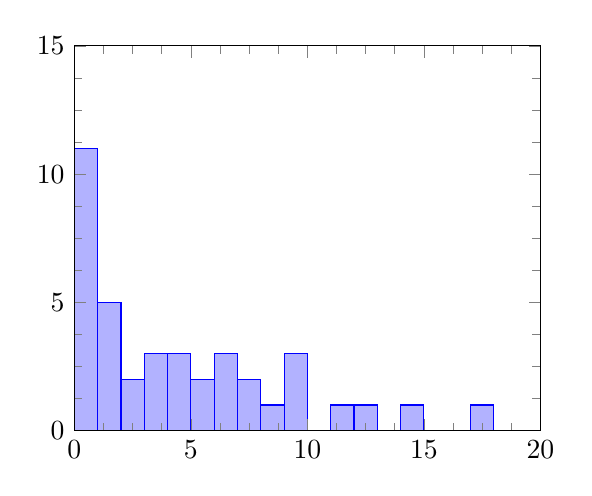
\begin{tikzpicture}
        \begin{axis}[
            ymin=0, ymax=15,
            xmin=0, xmax=20,
            minor y tick num = 3,
            minor x tick num = 3,
            area style,
            ]
        \addplot+[ybar interval, mark=no] plot coordinates { (0, 11) (1, 5) (2, 2) (3, 3) (4, 3) (5, 2) (6, 3) (7, 2) (8, 1) (9, 3) (10, 0) (11, 1) (12, 1) (13, 0) (14, 1) (15, 0) (16, 0) (17, 1) (18, 0) };
        \end{axis}
    \end{tikzpicture}
\end{center}

The mean is larger than the median since we have a right-skewed distribution with outliers.

\newpage

\item[2.6]
\begin{itemize}
\item[(a)]
The stemplot for the data of defensive linemen is
\item[]
\item[]

\begin{center}
\begin{tabular}{r | *{120}{c}}
    24 & 2\\
    25 & 2 & 4\\
    26 & 0\\
    27 & 4\\
    28 & \\
    29 & 7\\
    30 & 0 & 3\\
    31 & 1\\
    32 & 3
\end{tabular}
\end{center}

\item[]
\item[]
\textbf{\und{Five-number summary}}\\\\
Minimum is $242$.\\\\
$Q_1$ is $254$.\\\\
Median is $\dfrac{274 + 297}{2} = 285.5$.\\\\
$Q_3$ is $303$.\\\\
Maximum is $323$.

\item[]

\item[(b)]
The stemplot for the data of offensive linemen is
\item[]
\item[]
\begin{center}
    \begin{tabular}{r | *{120}{c}}
        29 & 8\\
        30 & 1 & 5\\
        31 & 0 & 5 & 8\\
        32 & 0 & 1\\
        33 & 2
    \end{tabular}
\end{center}
\item[]
\item[]

\textbf{\und{Five-number summary}}\\\\
Minimum is $298$.\\\\
$Q_1$ is $\dfrac{301 + 305}{2} = 303$.\\\\
Median is $315$.\\\\
$Q_3$ is $\dfrac{320 + 321}{2} = 320.5$.\\\\
Maximum is $332$.

\item[]

\item[(c)]
The stemplot for offensive linemen is symmetric and has
not outliers. The stemplot for defensive linemen is almost
symmetric and also does not have any outliers. The group
of offensive linemen are heavier since its datapoints have
higher values
\end{itemize}

\item[]
\item[]

\item[2.7]
\begin{itemize}
\item[(a)]
\textbf{\und{Five-number summary}}\\\\
Minimum is $11$.\\\\
$Q_1$ is $18$.\\\\
Median is $21$.\\\\
$Q_3$ is $26$.\\\\
Maximum is $51$.

\item[]

\item[(b)]
Here is the boxplot for the given data:
\item[]
\item[]
\begin{center}
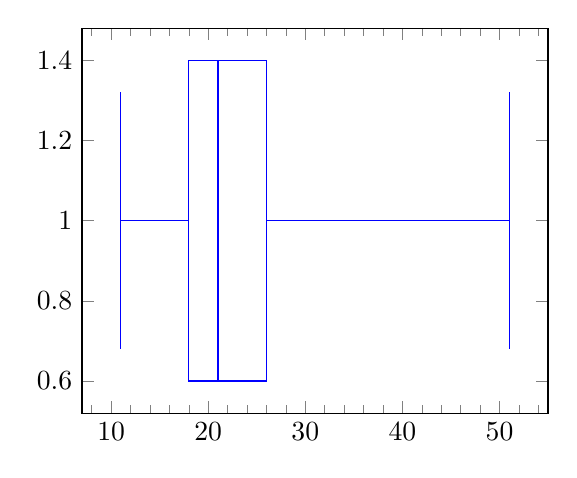
\begin{tikzpicture}
\begin{axis}
    [
    minor x tick num = 4,
    ]
    \addplot+[
    boxplot prepared={
    lower whisker=11,
    lower quartile=18,
    median=21,
    upper quartile=26,
    upper whisker=51
    },
    ] coordinates {};
\end{axis}
\end{tikzpicture}
\end{center}
\item[]
\item[]

It is easy to see that the distribution is right-skewed.
This is due to the box being more to the left of the graph.
There are no unusually small observations. There are
some unusually large observations, namely $43$, $45$, $47$,
$50$ and $51$.
\end{itemize}


\item[]
\item[]

\item[2.9]
\begin{itemize}
\item[$\bullet$]
Which of these are suspected outliers by the $1.5 \times \text{IQR}$ rule?
\begin{quote}
Notice that $1.5 \times \text{IQR} = 1.5 \times (26 - 18) = 12$ and therefore an outlier would be a datapoint
with the value less than $6$ or greater than $38$. Therefore, the outliers
would be the datapoints $40$, $40$, $40$, $43$, $45$, $47$, $50$, and $51$.
\end{quote}

\item[$\bullet$]
In this case, the cars producing the high outliers share a common feature.
What do you think that is?
\begin{quote}
There might be a lot of reasons actually. For instance, it might be that these
cars were malfunctioning (wrong gears, worn out tyres etc.) or it might be that
they were overspeeding etc.
\end{quote}
\end{itemize}

\item[]
\item[]

\item[2.10]
\begin{itemize}
\item[(a)]
$\dfrac{6.2 + 12.8 + 7.6 + 15.4}{4} = \dfrac{19 + 23}{4} = \dfrac{42}{4} = 10.5$.
\end{itemize}

\item[]

\item[(b)]
\begin{align*}
&s = \sqrt{\dfrac{1}{4 - 1}((10.5 - 6.2)^2 + (10.5 - 12.8)^2 + (10.5 - 7.6)^2 + (10.5 - 15.4)^2)}\\
&= \sqrt{\dfrac{1}{3}(4.3^2 + (-2.3)^2 + 2.9^2 + (-4.9)^2}\\
&= \sqrt{\dfrac{1}{3}(18.49 + 5.29 + 8.41 + 24.01)}\\
&= \sqrt{\dfrac{56.2}{3}} \approx \sqrt{18.73} \approx 4.327
\end{align*}

\item[]

\item[(c)]
I entered the data into the calculator and the results agree with my hand calculations.
Follow this link to verify -- \url{https://www.calculator.net/standard-deviation-calculator.html?numberinputs=6.2%2C+12.8%2C+7.6%2C+15.4&x=26&y=29}.

\item[]
\item[]

\item[2.11]
$\overline{x_A} \approx 7.5$ and $s_A \approx 2.03$.\\
$\overline{x_B} \approx 7.5$ and $s_B \approx 2.03$.\\\\
Indeed, $\overline{x_A} \approx \overline{x_B}$ and $s_A \approx s_B$.\\\\
Here are the stemplots for the datasets $A$ (to the left) and $B$ (to the right):
\item[]
\item[]
\begin{center}
    \begin{tabular}{r | *{120}{c}}
        Data A\\
        3 & 10\\
        4 & 74\\
        5 & \\
        6 & 13\\
        7 & 26\\
        8 & 10 & 14 & 74 & 77\\
        9 & 13 & 14 & 26
    \end{tabular}
    \qquad
    \begin{tabular}{r | *{120}{c}}
        Data B\\
        5 & 25 & 56 & 76\\
        6 & 58 & 89\\
        7 & 71 & 04 & 91\\
        8 & 47 & 84\\
        9 & \\
        10 & \\
        11 & \\
        12 & 50
    \end{tabular}
\end{center}
\item[]
where $3 \mid 10 = 3.10$, $4 \mid 74 = 4.74$ etc.
\item[]
Data $A$ is left-skewed while Data $B$ is right-skewed (also looks like uniform one with $50$ being an outlier).

\newpage

\item[2.12]
\begin{itemize}
\item[(a)]
No since the distribution is not symmetric.

\item[]

\item[(b)]
Yes since the distribution is symmetric.

\item[]

\item[(c)]
No since the distribution is not symmetric.
\end{itemize}

\item[]
\item[]

\item[2.13]
\begin{itemize}
\item[$\bullet$]
State: Is logging the cause of decline in number of trees?
\item[$\bullet$]
Plan: We have to find the mean and the standard deviation.
\item[$\bullet$]
Solve:
$\overline{x_{\text{Group 1}}} = 23.75$, $\overline{x_{\text{Group 2}}} = 14.08$, $\overline{x_{\text{Group 3}}} = 15.78$.\\
$s_{\text{Group 1}} = 5.06$, $s_{\text{Group 2}} = 4.98$, $s_{\text{Group 3}} = 5.76$.
\item[$\bullet$]
Conclude: It appears that logging indeed has a negative effect on the number of trees.
If no logging is present, the average number of trees is higher.
\end{itemize}

\item[]
\item[]

\item[2.29]
\begin{itemize}
\item[$\bullet$]
Do the boxplots fail to reveal any important information visible in the stemplots of Figure 2.5?
\begin{quote}
Generally speaking, no since the boxplot still shows us the shape of the distribution.
However, in this case, boxplots did not show the gap in the south between the rates of
DC and Georgia. Therefore, boxplots did not fail to show the general overview, but they
did fail to reveal some particular information.
\end{quote}
\item[$\bullet$]
Which plots make it simpler to compare the regions?
\begin{quote}
Boxplots since one could compare the spread and the center right away which is not
possible in stemplots.
\end{quote}
\end{itemize}

\item[]
\item[]

\item[33.]
\begin{itemize}
\item[(a)]
Symmetric distributions are best summarized with $\overline{x}$ and $s$.
Since the distribution in the exercise 1.38 is symmetric, $\overline{x}$
and $s$ are indeed appropriate measures in this case.

\item[]

\item[(b)]
With the datapoint $229$, we get that $\overline{x} \approx 59.71$ and $s \approx 63.03$.\\
Without the datapoint $229$, we get that $\overline{x} \approx 51.25$ and $s \approx 50.97$.\\\\
Hence, we got that the mean decreased by approximately $8.46$ and that the standard deviation
decreased by approximately $12.06$.

\item[]

\item[(c)]
With the outlier, we get that $M = 61$ and without it, we get that $M = 57.5$.
Therefore, we got that the median decreased by 3.5. Since the mean decreased
by approximately $8.46$ and the median decreased by $3.5$, it is clear that
the median is more resistant than the mean.
\end{itemize}

\end{itemize}
\end{document}
